\documentclass[12pt,a4paper,titlepage,twoside]{report}
% set line spacing to 1.5 and font to Times
\renewcommand{\baselinestretch}{1.5}
\usepackage{times}

\usepackage[
backend=biber,
style=ieee,
citestyle=ieee
]{biblatex}
\addbibresource{references.bib}

\usepackage{graphicx}
\usepackage[justification=centering]{caption}
\usepackage{subcaption}
\usepackage{amssymb}
\usepackage{bm}
\usepackage{pdfpages}
\usepackage{indentfirst}
\usepackage{underscore}
\usepackage{float} %figure inside minipage

\newcommand\todo[1]{\textcolor{red}{#1}}

\usepackage{anysize}
\marginsize{2.5cm}{2.5cm}{2.5cm}{2.5cm}

\usepackage[pagestyles]{titlesec}
\titleformat{\chapter}{\normalfont\huge}{\thechapter.}{20pt}{\huge}
\titlespacing*{\chapter}{0pt}{-50pt}{40pt}

\newpagestyle{no-chapter-headers}{
  \sethead[\thepage][][\chaptertitle]  				% even pages
  		  {\thesection~\sectiontitle}{}{\thepage}	% odd pages
}
\pagestyle{no-chapter-headers}

% Front title sheet containing following information:
%	Name, I.D. number, Supervisor's Name, Course Followed, Year, Department, Title of Project.
\title{
  
\includegraphics[width=0.3\linewidth]{./images/ul-logo.jpg}
  \hspace{1cm}
  
\includegraphics[width=0.6\linewidth]{./images/ECE_Logo.png}
  %\centering
\includegraphics[width=14cm]{ECE_Logo.png}\\ [2ex]
  Machine Learning Using Python Frameworks
}
\author{Lorcan Williamson\\Supervisor: Dr. K. Murphy}

\begin{document}

\maketitle

% An abstract of not more than 200 words
\begin{abstract}
	Machine learning and deep learning have advance rapidly in recent years due to the increase computing power and availability. Python is a popular language choice for machine learning tasks, with a number of frameworks available for the development of machine and deep learning models. This project aims to look at how code is developed using these frameworks, and compare their functionality to those in other languages.
\end{abstract}

% Table of contents
\tableofcontents
\newpage

% Introduction 
% 	Clearly stating the objectives of the project and may include material from the report submitted in the Autumn semester
\chapter{Introduction}
	
	The aim of this project was to look at machine and deep learning frameworks in Python and the code development process to build and train various ML/DL models using them. To this end 3 of the main machine learning frameworks were looked at: Scikit-learn\cite{scikit-learn}; TensorFlow\cite{tensorflow}; and Keras\cite{keras}, using TensorFlow for the backend. Initially 3 example problems were looked at to demonstrate the various features of these frameworks, but this was changed to 2 afterwards due to time constraints. These two problems being:
	\begin{itemize}
	\item \textbf{Predicting student test performance}: The goal of this example was to predict the test scores of students based on a number of factors. This problem aimed to cover a variety of common machine learning models such as Support Vector Machines, Decision Trees, Random Forests and Multi-Layer Perceptrons. The work done for this example loosely followed the work done in the paper this data was originally collected for \textit{Using Data Mining To Predict Secondary School Student Performance}\cite{student-dataset}. The data mining models for this were developed using R, so this also allows for a comparison between Python and R machine learning frameworks.
	\item \textbf{Detecting pneumonia in chest x-rays}: The goal of the second example was to detect whether pneumonia was present in a chest x-ray or not. This would allow for a look at Convolutional Neural Networks, a deep learning model that has only really become common in the last decade due to the computational power and amount of data required to train them. The data for this problem came from \textit{Labeled Optical Coherence Tomography (OCT) and Chest X-Ray Images for Classification}\cite{pne-dataset}.
	\end{itemize}
	Code for this project was developed using the following frameworks and technologies:
	\begin{itemize}
	\item Python (version 3.6)
	\item Scikit-learn (version 0.21.3)
	\item Keras (version 2.2.4 (TensorFlow version 1.13.1 backend))
	\item AWS EC2 instance (Hardware instance: p2.xlarge, running: Deep Learning AMI (Ubuntu) Version 24.1)
	\end{itemize}
	
	
\chapter{Problem 1: Predicting Student test Scores}

\section{Problem Background}
	 The goal of this problem was to look at how various machine learning models are implemented using Python frameworks. For this problem 4 types of ML models were looked at: SVMs; DTs; RFs; and NNs. These were implemented using the Scikit-learn and Tensorflow frameworks. These models were chosen as they were used in the original paper looking at this dataset\cite{student-dataset}. The original paper used R to develop their models. By using similar models and methodology a caparison can be made between the functionality of the python frameworks and those in R using the RMiner framework. 
	
\section{Dataset}
	The dataset used consists of 2 csv files corresponding to the two subjects data was collected for, Mathematics and Portuguese. Both files have 33 columns, explained in table 1, corresponding to the 32 features of the dataset, and 1 label. Each entry in the files corresponds to a student, some students appear in both files. There are 649 students represented in the Portuguese data, and 396 students in the Mathematics file. For this reason the Portuguese subject data was used for training and testing the models. Before the data was used for training it had to be preprocessed. All the non-numeric features, such as \textit{school} and \textit{Mjob} were converted to numeric using a one-hot-label encoding.  This preprocessing was done using Scikit-learns \texttt{sklearn.preprocessing.LabelEncoder}. In Paulo Cortez and Alice Silva's original paper\cite{student-dataset} they looked at three different prediction metrics: binary pass/fail classification; 5 grade classification using the Erasmus grading scale; and regression using the 20 grade levels in the Portuguese education system. For this project only the 5 level classification was looked at. This meant that the 20 grades in the original data needed to be converted to the 5 Erasmus grades, using the following mapping: $16-20 :\rightarrow 5 (A), 14-15 :\rightarrow 4 (B), 12-13 :\rightarrow 3 (C), 10-11 :\rightarrow 2 (D), 0-9 :\rightarrow 1 (F)$
	\begin{figure}[t]
  		\centering
  		\includegraphics[width=\linewidth]{./images/student-table.png}
  		\captionof{table}{Student data available}
  		\label{fig:student-data}
	\end{figure}\\

\section{Implementations}
	For this problem the methodology of Paulo Cortez and Alice Silva's original paper was followed, and then expanded upon to try improve the results. In the original paper 4 machine learning models were looked at, SVMs, DT, RF and ANN. All these models were trained using 10-fold cross-validation, where the average validation accuracy was taken as the test accuracy. This was repeated 20 times for each model and the average accuracy and standard deviation was recorded. For this project the same 4 models were looked at, and trained with 10-fold cross-validation, but this was only done once for each model, and the average validation accuracy was compared to the expected. New models were then trained using data with extra processing, or with different hyper-parameters to try achieve better accuracy. The models were also tested on the maths dataset to see if they could perform well on unseen data from a different subject.

\subsection{Neural Network}

\subsubsection*{Overview}
	A neural network is a machine made up of many artificial neurons. The basic model for an artificial neuron was described by McCulloch and Pitts in 1943\cite{mcculloch-pitts-neuron}, Figure~\ref{fig:m-p-neuron}. The McCulloch-Pitts neuron works by taking the weighted sum of the inputs, and putting this through some activation function which produces an activation level for the neuron. A number of functions can be used for the activation, though rectified linear (relu) has become a common standard in recent years\cite{relu-activation}.
	\begin{figure}[h]
  		\centering
  		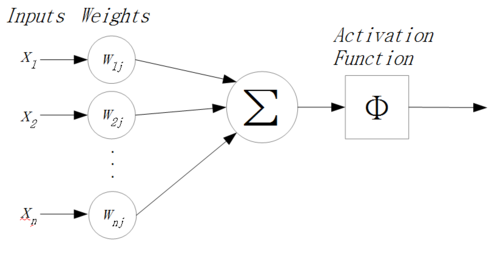
\includegraphics[width=0.7\linewidth]{./images/mcculloch-pitts.png}
		\caption{The McCulloch-Pitts neuron}
		\label{fig:m-p-neuron}
	\end{figure}\\
	The architecture of the model described in the paper was that of a multi-layer perceptron (MLP). This is a neural network made up of only dense layers\cite{intro-to-nn}. The MLP described was made up of an: input layer; a hidden layer with $H$ neurons; and an output layer. The hyper-parameter $H$ was optimized using grid search where $H \in \{0, 2, 4, 6, 8\}$. The model was trained using the BFGS\cite{bfgs} optimizer algorithm for 100 epochs, the defaults for the \texttt{nnet} package, the neural network package used by RMiner.
	\begin{figure}[h]
		\centering
		\includegraphics[width=0.7\linewidth]{./images/mlp-coloured.png}
		\caption{Multi-layer Perceptron architecture}
		\label{fig:mlp-fig}
	\end{figure}
	
\subsubsection*{Code Development}
	Code for this model was initially planned to be developed using the Keras API with a TensorFlow backend. However Keras has no built in BFGS optimizer. This meant base TensorFlow would need to be used as it easier to implement new optimisers. As the paper did not specify the loss function the mean squared error (MSE) was used\footnote{Implemented using \texttt{tf.keras.losses.MeanSquaredError()}} as it is the default for RMiner. The \texttt{tfp.optimizer.bfgs_minimize} function from the TensorFlow Probability library was used to minimize the loss function of the model. This function takes two positional arguments:
	\begin{itemize}
	\item \textbf{\texttt{value_and_gradients_function}}: A Python callable which takes a point (1D tensor) as input and returns the value of the function to be minimised and its gradient at that point.
	\item \textbf{\texttt{initial_position}}: The starting position of the function.
	\end{itemize}	
	One problem encountered was the fact that this function uses a single 1D tensor for the variable of the function, while the model uses multiple 2D tensors for the weights of the MLP. To solve this the 4 'weight' tensors\footnote{2 weight matrices  and 2 bias vectors} were mapped to and from a 1D tensor using TensorFlows \texttt{dynamic_stitch} and \texttt{dynamic_partition}. A blog post by Py Chuang implementing a similar optimizer was used as reference\cite{pychoa-optimizer} for creating the value_and_gradient function. \par
	For my implementation I decided to extend \texttt{tf.keras.Sequential} and create a \texttt{BfgsMlp} class, which creates MLP with a single hidden layer. This overrides the \texttt{fit} method from \texttt{Sequential} to use the \texttt{bfgs_minimize} optimizer. A number of extra methods were also added to facilitate its use:
	\begin{itemize}
	\item \textbf{\texttt{_make_val_and_grad_func(self, X, y)}}: A factory function to make the value_and_gradient function , which calculates the loss and gradient of the error surface for presentations X with labels y.
	\item \textbf{\texttt{_update_weights(self, weights_1d)}}: Updates the model weights using a 1D tensor calculated by the optimizer
	\item \textbf{\texttt{_get_weights_1d(self)}}: Gets the current weights for the model mapped to a 1D tensor
	\item \textbf{\texttt{_make_1d_mapping(self)}}: Called by \texttt{__init__} to create a mapping to and from a 1D tensor for the model weights.
	\end{itemize}
	Using this model the hyper-parameter $H$ was then tuned using 10-fold cross-validation, with the average validation accuracy for each value of $H$ recorded (See results section). Once the best value of $H$ was determined, the progression of the training and validation loss and accuracy over the 100 epochs. There was a problem with this however, as the BFGS optimizer does not return intermediate values, and weights need to be updated in the \texttt{value_and_gradient} function. To monitor the intermediate loss and accuracy of the model, a new class, \texttt{BfgsTrainingMonitor}, was made. This takes the model and the datasets you want to test the model with each epoch, i.e. the training and validation datasets. This monitor can then be passed to the \texttt{BfgsMlp.fit function}, and uses a wrapper function \texttt{monitor(func)} to wrap the value_and_gradient function for the model. It then calls the models \texttt{evaluate(X, y)} function, and records the results for the metrics returned in a Python dictionary. This was used to create graphs to show how the accuracy and loss change by epoch, see Figure~\ref{fig:nn-loss-acc}. There was one issue with this method however, which is that the value_and_gradient function appears to be called 3 times per iteration of the bfgs algorithm. I could not find any reason for this either in the TensorFlow Probability documentation for this function, or its source code. \par
	From these graphs it can be seen that after around 40 epochs the training loss continues to reduce while the validation loss begins increasing. This is a common sign that the model is overfitting and learning the noise of the training data, rather than the underlying information\cite{overfitting}. Using 40 epochs and 4 hidden neurons 5 final models was trained on 90\% of the Portuguese data, and validation accuracy calculated using the other 10\% of the data. The best model was then tested against the Maths data, and an accuracy of 65.32\% achieved.

\subsubsection*{Results}
	\begin{figure}[h]
		\centering
		\begin{subfigure}{0.5\textwidth}
	  		\centering
  			\includegraphics[width=\linewidth]{./images/nn-loss.png}
  			\caption{Training vs. Validation loss}
  			\label{fig:nn-loss}
		\end{subfigure}%
		\begin{subfigure}{0.5\textwidth}
  			\centering
	  		\includegraphics[width=\linewidth]{./images/nn-acc.png}
  			\caption{Training vs. Validation accuracy}
 			\label{fig:nn-acc}
		\end{subfigure}
		\caption{Training history for BfgsMlp with $H = 4$.\\ \small{Note No. calls to val_and_grad_func is 3x No. epochs}}
		\label{fig:nn-loss-acc}
	\end{figure}
	
	\begin{tabular}{r c c c c c}
	\hline
	\textbf{H}	& 0 & 2 & 4 & 6 & 8 \\ \hline
	\textbf{Accuracy} & 28.92\% & 66.15\% & 67.85\% & 62.15\% & 64.62\%  \\ \hline
	\end{tabular}

\subsection{Support Vector Machine}

\subsubsection*{Overview}
	Support vector machines (SVMs) were first described in 1995 by Corinna Cortes and Vladimir Vapnik in their paper \textit{Support-Vector Networks}\cite{support-vector-machines}. They are a popular machine learning algorithm as they reach a global optimum by maximising the distance between data points and the decision boundary, Figure~\ref{fig:svm-opt-bound}. SVMs allow for binary classification, though a multi-class SVM can be made from the combination of multiple binary SVMs, or using multi-class kernel-based vector machines\cite{multiclass-svm}. By themselves SVMs aren't of much use, as they can only solve linearly-separable problems. But by the use of the \textit{'kernel trick'}\cite{ml-algorithmic-perspective}. This uses  a kernel function to map the features into some higher dimensional space, where they are linearly-separable. \par
	SVMs offer a number of hyper-parameters, such as: \textbf{$C$} a 'slack' variable; and $\gamma$ a parameter used by the kernel functions. Only $\gamma$ was tuned in the original paper, where $\gamma \in \{2^{-9}, 2^{-7}, 2^{-5}, 2^{-3}, 2^{-1}\}$. The slack variable $C$ was left as the default value of 1, which is also the default in Scikit-Learn. No kernel was mentioned in the original paper, so several kernel functions were looked at: Radial-bias function (RBF); Sigmoid; Polynomial (degree 3); and linear, which does not map the data-points to a higher dimensionality space. No form of dimensionality reduction for the data such as principle component analysis (PCA) was looked at either, though it has been shown that removing features with little correlation to the labels can improve SVM classification performance\cite{svm-reduce-dim}. For this reason it was looked at to demonstrate Scikit-Learns various dimensionality reduction methods, and to see if it has any improvement on classification accuracy.
	\begin{figure}[h]
		\centering
  		\includegraphics[width=0.7\linewidth]{./images/temp.png}
  		\caption{Optimal decision boundary made by SVM}
  		\label{fig:svm-opt-bound}
	\end{figure}
	
\subsubsection*{Code Development}
	Code for this model was made using Scikit-Learn's \texttt{sklearn.svm.SVC} class. To tune the $\gamma$ value, scikit-learn's \texttt{sklearn.model_selection.GridSearchCV} was used. This allows for a user to tune a models hyper-parameter using a grid-search method, i.e. checking all combinations of hyper-parameters, and using k-fold cross-validation to measure performance. Hyper-parameters are given in a Python dictionary, along model and some training data. Once training of the models is done, various information about the results can be accessed, along with the best performing model. For this grid-search, both the $\gamma$ value and the kernel functions were varied. The results for this can be seen in Tables~\ref{tab:no-pca-tab}--~\ref{tab:scree-pca-tab} in the SVM results section. \par
	Next the affect of reducing dimensionality on the accuracy of the classification was looked at. For this a number of PCA algorithms were looked at. Principle component analysis, as the name suggests, looks at the variance captured in each feature, and continues to take the feature which represents the most variance, until a certain threshold is reached\cite{pca}. The remaining features are then discarded, and the the selected features used as the new dataset. This also corresponds to taking the $q$ largest eigenvectors of the data's covariance matrix, and this the method implemented by Scikit-Learn. There are numerous ways to select how many PCs should be used, such as Kaiser's stopping rule or the scree test\cite{pca-choosing}. Kaiser's stopping rule states that only factors with an eigenvalue of greater than $1.00$ should be used. Table~\ref{tab:kaiser-tab} shows the top 11 eigenvalues, of these 10 would be used as they are greater than $1$. The scree test takes a more graphical approach to this, by plotting the features vs. their eigenvalues in descending order, it can be seen when the eigenvalues level out, and this is taken as the cut-off, as seen in Figure~\ref{fig:scree-test}, this happens after the first 3 features. An identical approach was then used to performing hyper-parameter tuning for the models using datasets of this dimensionality.\\
	\begin{minipage}[t]{\textwidth}	
		\begin{minipage}{0.3\textwidth}
		\begin{table}[H]
			\centering
			\begin{tabular}{|r|r|}
				\hline
				\textbf{Factor} & \textbf{Eigenvalue} \\ \hline
				1	&	3.8335 \\
				2	&	2.5561 \\
				3	&	1.7764 \\
				4	&	1.5177 \\
				5	&	1.4267 \\
				6	&	1.3117 \\
				7	&	1.2629 \\
				8	&	1.1248 \\
				9	&	1.0694 \\
				10 	&	1.0327 \\
				11	&   0.9958 \\
				\hline
			\end{tabular}
			\caption {Factors and Eigenvalues} 
			\label{tab:kaiser-tab} 
		\end{table}
		\end{minipage}%
		\hspace{0.6cm}%
		\begin{minipage}{0.7\textwidth}
		\begin{figure}[H]
			\centering
			\vspace{0.9cm}
			\includegraphics[width=\textwidth]{./images/scree-test.png}
			\caption{Scree Test showing factor vs. eigenvalue. Notice the drop off after 3 factors}
			\label{fig:scree-test}
		\end{figure}
		\end{minipage}
	\end{minipage} \\
	
\subsubsection*{Results}
	For the first test ,not using PCA on the data, it was found that setting the kernel to 'linear', i.e. using no kernel function, got the best result and was closest to the result in the original paper, with a mean accuracy of $67.62\% \pm4.8$. This is unexpected, as the best model with a kernel function only had a mean accuracy of $51.73\% \pm4.3$, with a $\gamma$ of 0.002. It also means that $\gamma$ was unused by the best model, so tuning it was not needed. It can also be seen for all data inputs, Tables~\ref{tab:no-pca-tab} -- \ref{tab:scree-pca-tab}, that for $\gamma < 2^{-5}$ no difference was seen in accuracy for any kernel.\\
	\begin{table}[h]
		\centering
		\begin{tabular}{|ll|ccccc|}
			\hline
                                      &                                      &   			& \multicolumn{3}{c}{\textbf{Gamma $\boldsymbol{\gamma}$}} &   \\ \hline
                                      &                                      				& $2^{-9}$  		& $2^{-7}$       	& $2^{-5}$      	& $2^{-3}$			& $2^{-1}$ \\ \hline
			\multicolumn{1}{|l|}{\textbf{Kernel}} & \multicolumn{1}{r|}{\textbf{Linear}} 	& \boldmath$67.62\% \pm4.8$ 	& --  	& --				& --	  			& --			   \\
			\multicolumn{1}{|l|}{\textbf{}}       & \multicolumn{1}{r|}{\textbf{RBF}}    	& $31.84\% \pm0.7$ 	& $31.84\% \pm0.7$  & $31.84\% \pm0.7$  & $45.23\% \pm6.6$  & $32.37\% \pm2.0$ \\
			\multicolumn{1}{|l|}{\textbf{}}       & \multicolumn{1}{r|}{\textbf{Poly}}   	& $31.84\% \pm0.7$ 	& $31.84\% \pm0.7$  & $31.84\% \pm0.7$  & $31.84\% \pm0.7$  & $50.02\% \pm6.5$ \\
			\multicolumn{1}{|l|}{\textbf{}}       & \textbf{Sigmoid}                     	& $31.84\% \pm0.7$ 	& $31.84\% \pm0.7$  & $31.84\% \pm0.7$  & $38.00\% \pm4.9$  & $51.73\% \pm4.4$ \\ \hline
		\end{tabular}%
		\caption {Results using no PCA (Best accuracy in bold)} 
		\label{tab:no-pca-tab} 
	\end{table}
	
	\begin{table}[h]
		\centering
		\begin{tabular}{|ll|ccccc|}
			\hline
                                      &                                      &   			& \multicolumn{3}{c}{\textbf{Gamma $\boldsymbol{\gamma}$}} &   \\ \hline
                                      &                                      				& $2^{-9}$  		& $2^{-7}$       	& $2^{-5}$      	& $2^{-3}$			& $2^{-1}$ \\ \hline
			\multicolumn{1}{|l|}{\textbf{Kernel}} & \multicolumn{1}{r|}{\textbf{Linear}} 	& \boldmath$56.51\% \pm4.8$ 	& --  	& --				& --	  			& --			   \\
			\multicolumn{1}{|l|}{\textbf{}}       & \multicolumn{1}{r|}{\textbf{RBF}}    	& $31.84\% \pm0.7$ 	& $31.84\% \pm0.7$  & $31.84\% \pm0.7$  & $41.81\% \pm5.2$  & $47.93\% \pm6.2$ \\
			\multicolumn{1}{|l|}{\textbf{}}       & \multicolumn{1}{r|}{\textbf{Poly}}   	& $31.84\% \pm0.7$ 	& $31.84\% \pm0.7$  & $31.84\% \pm0.7$  & $31.84\% \pm0.7$  & $46.75\% \pm7.2$ \\
			\multicolumn{1}{|l|}{\textbf{}}       & \textbf{Sigmoid}                     	& $31.84\% \pm0.7$ 	& $31.84\% \pm0.7$  & $31.84\% \pm0.7$  & $37.66\% \pm4.3$  & $48.29\% \pm6.5$ \\ \hline
		\end{tabular}%
		\caption {Results using Kaiser PC selection (Best accuracy in bold)} 
		\label{tab:kasier-pca-tab}
	\end{table}
	
	\begin{table}[h!]
		\centering
		\begin{tabular}{|ll|ccccc|}
			\hline
                                      &                                      &   			& \multicolumn{3}{c}{\textbf{Gamma $\boldsymbol{\gamma}$}} &   \\ \hline
                                      &                                      				& $2^{-9}$  		& $2^{-7}$       	& $2^{-5}$      	& $2^{-3}$			& $2^{-1}$ \\ \hline
			\multicolumn{1}{|l|}{\textbf{Kernel}} & \multicolumn{1}{r|}{\textbf{Linear}} 	& $45.54\% \pm6.2$ 	& --  				& --				& --	  			& --			   \\
			\multicolumn{1}{|l|}{\textbf{}}       & \multicolumn{1}{r|}{\textbf{RBF}}    	& $31.84\% \pm0.7$ 	& $31.84\% \pm0.7$  & $31.84\% \pm0.7$  & $40.77\% \pm5.1$  & \boldmath$46.39\% \pm6.1$ \\
			\multicolumn{1}{|l|}{\textbf{}}       & \multicolumn{1}{r|}{\textbf{Poly}}   	& $31.84\% \pm0.7$ 	& $31.84\% \pm0.7$  & $31.84\% \pm0.7$  & $31.84\% \pm0.7$  & $42.47\% \pm7.0$ \\
			\multicolumn{1}{|l|}{\textbf{}}       & \textbf{Sigmoid}                     	& $31.84\% \pm0.7$ 	& $31.84\% \pm0.7$  & $31.84\% \pm0.7$  & $37.14\% \pm3.9$  & $33.08\% \pm6.1$ \\ \hline
		\end{tabular}%
		\caption {Results using Scree PC selection (Best accuracy in bold)} 
		\label{tab:scree-pca-tab}
	\end{table} \par
	As mentioned, removing features from the data with little correlation can improve the accuracy of SVMs. For this data however this was not the case, both Kaiser and Scree principle component selections achieved worse accuracy. This is because as seen Figure~\ref{fig:scree-test}, the majority of principle components had an eigenvalue of greater than 0.5, and thus were non-negligible in terms of the amount of variance they represented. Thi can be seen more clearly in Figure~\ref{fig:pca-variance}, which shows that each feature explains about an equal percent of the variance, indicated by the plot being close to linear. \par
	However there is another benefit of reducing dimensionality, which is the reduction to training times. Using the full 32 features of the training set, it took 0.04 seconds to train and model using a linear kernel on average, compared to 0.014 seconds when using 10 features and 0.009 seconds when using 3 features. While for a dataset of this size training time is not an issue, for datasets that could have over a 100,000 presentations this could represent reasonable trade-off in accuracy for training time, especially if features with low variance exist in the dataset.
	\begin{figure}[h]
		\centering
		\includegraphics[width=0.7\linewidth]{./images/pca-variance.png}
		\caption{Plot showing accumulative explained variance for the principle components (Blue) \\Orange represents perfectly equal explained variance by each PC}
		\label{fig:pca-variance}
	\end{figure}
	
\subsection{Decision Tree}
	
\subsubsection*{Overview}
	Binary trees are a very common and well studied data-structure in computer science. Searching through a balanced binary tree is very efficient, $O(\log N)$, where $N$ is the number of nodes. Decision trees are binary trees constructed to classify data based on features\cite{ml-algorithmic-perspective}. This makes them very fast for querying once they have been constructed. There are a number of algorithms for constructing decision trees, such as ID3\cite{ID3} or CART\cite{CART}. These are usually greedy algorithms that focus on trying to separate the features to split the classes the most evenly. To do this they use some measure of informational entropy, which measures how much the data can be split by a single feature, which is a maximum when it splits the data is split in half\cite{info-entropy}. \par
	The default entropy function used by the \texttt{rpart} models, the decision tree package used by \texttt{rminer} is Gini impurity, Eqn.~\ref{eqn:gini}, which is the entropy measurement used by CART. This function computes the \textit{'purity'} of a node, where a pure node is one that corresponds to a single class $i$ in the dataset, if that node where to split the data based on some feature $k$. If we count the number of data points $N(i)$ then we can calculate the Gini impurity as:
	\begin{equation}
	G_k = 1 - \sum_{i=1}^c N(i)^2
	\label{eqn:gini}
	\end{equation}
	Along with the criterion function on which nodes are split, there are a number of other hyper-parameters that can be used to improve decision tree performance. Of particular importance to preventing over-fitting are the maximum depth of the decision tree, and the \textit{complexity parameter} used in minimal cost-complexity pruning. The maximum depth, as the name suggests, simply limits the maximum number of layers a decision tree can have. This stops the tree from splitting features too many times to try and correctly classify every point. Minimal cost-complexity pruning is an algorithm for pruning nodes from trees to minimise $R_\alpha(T)$, where $\alpha \geq 0$ is the complexity parameter (Eqn.~\ref{eqn:ccp}). Here $R(T)$ is the is the total misclassification rate of tree $T$, and $|T|$ is the number of terminal nodes in $T$.
	\begin{equation}
	R_\alpha(T) = R(T) + \alpha|T|
	\label{eqn:ccp}
	\end{equation}
	
\subsubsection*{Code Development}
	For tuning the max depth and the complexity parameter of the decision tree \texttt{GridSearchCV} was again used. While \texttt{rpart} supports both of these hyper-parameters, it does not have default values for them, and none was mentioned in the paper. For this reason the grid-search was set to tune the \texttt{max_depth} and the \texttt{ccp_alpha} hyper-parameters of the \texttt{DecisionTreeClassifier} from Scikit-learn. The max depth was tried with 3 different values, 3, 5, and None. For the complexity parameter two values were tested, 0, and the optimal $\alpha$ value. The optimal $\alpha$ value was calculated as follows:
	
	\begin{enumerate}
	\item Using \texttt{DecisionTreeClassifier.cost_complexity_pruning_path(X, y)} the effective $\alpha$ of each node in a tree can be calculated. This is the $\alpha$ at which the node would be pruned from the tree. 
	\item From these effective alphas we can create DTs using these values and plot the number of nodes and depth of the tree's against $\alpha$, as seen in Figure~\ref{fig:alpha-nodes-depth}, the depth and number of nodes quickly drop off as $\alpha$ increases.
	\item Using these models we can also plot the training and validation accuracy against $\alpha$, as seen in Figure \ref{fig:alpha-accuracy}. From this the best $\alpha$ to prevent over-fitting can be seen to be around 0.005. This value maximises validation accuracy, and as seen in Figure~\ref{fig:alpha-nodes-depth} also reduces the number of nodes and the depth drastically, improving generalisation of the trees.
	\end{enumerate}
	
	The two best trees were then graphed using \texttt{sklearn.tree.export_graphviz} and \texttt{graphviz}. These can be seen in Figures \ref{fig:dt-no-ccp} and \ref{fig:dt-ccp}. These offer an easy way to see how the data is being split at each node, and the effect of cost-complexity pruning on a decision tree\footnote{A full page version of these trees can be seen in the appendix, as they are quite large}. The colour each node corresponds to the dominant class at that node, with shade corresponding to the proportion of data points of that class at that node. From these it can be seen how cost-complexity pruning reduces the number of terminal nodes.
	
	\begin{minipage}[t]{\textwidth}
	\begin{minipage}{0.5\textwidth}
		\centering
		\begin{figure}[H]
	  		\centering
  			\includegraphics[width=\linewidth]{./images/node-alpha.png}
  			\caption{$\alpha$ vs. Size of tree}
  			\label{fig:alpha-nodes-depth}
		\end{figure}
	\end{minipage}%
	\hspace{0.5cm}%
	\begin{minipage}{0.5\textwidth}
		\begin{figure}[H]
  			\centering
	  		\includegraphics[width=\linewidth]{./images/alpha-acc.png}
  			\caption{$\alpha$ vs. Training and Validation accuracy}
 			\label{fig:alpha-accuracy}
		\end{figure}
	\end{minipage}%
	\hspace{0.5cm}
	\end{minipage}
	
	\begin{figure}[h]
		\centering
  		\includegraphics[width=\linewidth]{./images/dt-no-ccp.png}
  		\caption{Best decision tree without pruning}
  		\label{fig:dt-no-ccp}
	\end{figure}
	
	\begin{figure}[h]
		\centering
  		\includegraphics[width=\linewidth]{./images/dt-ccp.png}
  		\caption{Best decision tree with pruning}
  		\label{fig:dt-ccp}
	\end{figure}
	
\subsubsection*{Results}
	The results from the hyper-parameter grid-search using 10-fold cross-validation can be seen below, Table \ref{tab:dt-results}. From this a number of observations can be made about the effect of both the max depth and $\alpha$ value have on a decision tree's accuracy and training time. The first observation is that both limiting the max depth and using cost-complexity pruning improve validation results greatly. Without pruning limiting the max depth improves validation accuracy by around 14\%, and without limiting the depth pruning improves the validation accuracy by around 11\%. However it is also seen that the combination of limiting depth and pruning does not improve the validation much compared to the use of just on of these techniques, only around 0.5\%. 
	
	\begin{table}[h]
		\centering
		\begin{tabular}{|c|c|c|c|c|}
			\hline
			\textbf{Max Depth} 	& $\boldsymbol{\alpha}$ & \textbf{Mean fit time} (s) 	& \textbf{Mean accuracy} 	& \textbf{Standard deviation}	\\ 
			\hline
			3					& 0			& 0.0000						& 75.83\%					& 5.6\%	\\
			5					& 0			& 0.0020						& 68.28\%					& 6.5\%	\\
			--					& 0			& 0.0038						& 61.25\%					& 9.2\% \\
			\textbf{3}			& \textbf{0.005}& \textbf{0.0025}			& \textbf{76.34\%}			& \textbf{5.8\%} \\
			5					& 0.005		& 0.0032						& 73.93\%					& 7.2\% \\
			--					& 0.005		& 0.0050						& 72.38\%					& 9.1\% \\
			\hline
		\end{tabular}
		\caption{GridSearchCV results}
		\label{tab:dt-results}
	\end{table}
	
	The best model with and without pruning were then evaluated using the unseen maths dataset. With pruning an accuracy of 74.94\% was measured on the unseen data, compared to 71.39\% with pruning.
	
\subsection{Random Forest}

\subsubsection*{Overview}
	Random forests are a type of ensemble learner made up of decision trees. Ensemble learners work by taking a large number, of weak learners\footnote{A weak learner is a model whose accuracy is slightly better than chance}, each classifying the data in a different way, and combining there predictions using some algorithm\cite{ml-algorithmic-perspective}. To create a random forest the method of training the decision trees is modified slightly. Now when a node is expanded only some subset of features $m$ is considered to split the data on. The trees are then trained and combined using bootstrap-aggregation, also known as bagging. Bootstrapping involves taking some random subset of the dataset with replacement. A number of these bootstrap samples are combined to produce a new dataset of the same size as the original dataset, but that may now contain duplicates. \par
	Again the original paper used the defaults for training the RF. The RF used by \texttt{rminer} comes from the \texttt{randomForest} package in R. This defaults to 500 trees, and a minimum node size of 1 for classification. Node size refers to the number of data points associated with a node. This parameter is equivalent to the \texttt{min_samples_leaf} in Scikit-learn's \texttt{RandomForestClassifier}. However the size of the trees can also be limited by the \texttt{max_depth} parameter. Scikit-learn uses 100 trees with no max depth if the default options are used. It was decided to see how 100 trees perform in this task compared to 500. As neither library limits the size of the trees by default, and producing 100's of large trees will take significant time, it was decided to also seem how limiting the size using both \texttt{max_depth} and the \texttt{min_samples_leaf} of the trees affected the accuracy. This was checked using a grid-search method.
	
\subsubsection*{Code Development}
	As hyper-parameters were to be tuned using a grid-search method, \texttt{GridSearchCV} was again used. The \texttt{min_samples_leaf} argument can take either an integer value, or a float, depending on if it should be interpreted as the absolute number or a proportion of the total dataset. Here the hyper-parameters to be tuned were $\texttt{n_estimators} \in \{100, 500\}$, $\texttt{max_depth} \in \{3, \texttt{None}\}$ and $\texttt{nim_samples_leaf} \in \{1, 0.05\}$. 
	
\subsubsection*{Results}

	\begin{table}
		\centering
		\begin{tabular}{|c|c|c|c|c|}
			\hline
			\textbf{Max Depth} 	& \textbf{No. Estimators} & \textbf{Mean fit time} (s) 	& \textbf{Mean accuracy} 	& \textbf{Standard deviation}	\\ 
			\hline
			3 		& 100 	& 0.165 	& 67.03\%  & 5.4\% \\
			3 		& 500 	& 0.845 	& 68.42\%  & 5.5\% \\
			None 	& 100 	& 0.214 	& 69.48\%  & 5.3\% \\
			None 	& 500 	& 1.076 	& 71.32\%  & 6.6\% \\
			\hline
		\end{tabular}
	\end{table}
	
\subsection{Comparison of Results}

\chapter{Problem 2: Detecting Pneumonia}
\section{Problem Overview}
	% Explanation of pneumonia
	Pneumonia is an inflammation of the lungs which can be caused by either a fungal, bacterial or viral infection. Of these bacterial or viral infection are the more common cause\todo{source}. According to the \textit{The European Lung white book; Respiratory Health and Disease in Europe} it had a mortality rate in Ireland of 32.96 per 100,000 in 2011\cite{pne-death-rate}, which, when compared to the total death rate in Ireland for 2011 of 6.2 per 1,000, means that pneumonia was responsible for 5.3\% of deaths in Ireland in 2011. \todo{More prevalent in children and elderly}. \par
	% Diagnosis mehtods and use of deep learning in medicine
	There are a number of methods to reliably rule in or out pneumonia when diagnosing a patient, such as the lack of certain symptoms or the presence of rates and bronchial breathing sounds, but chest radiography is generally considered the best method of confirming a pneumonia diagnosis\cite{pne-diagnosis}. There has been a great amount of research into the use of deep learning in medical diagnosis in recent years, in particular for use image-based diagnosis, such as MRI, CAT or X-Rays\cite{pne-ml-in-medicine}. \todo{Examples of ML for diagnosis}. These models are often able to achieve comparable, or sometimes higher, detection rates of these diseases compared to doctors, making them very useful tools. \par
	% Details on dataset
	This example problem aims to demonstrate how a machine learning model could be developed for detecting pneumonia from chest x-rays. A number of deep learning methods will be explored, but only convolutional neural network (CNNs) models will be used, as almost all real world models for image-based medical diagnosis use CNNs\cite{pne-ml-in-medicine}. \par

\section{Convolutional Neural Networks}
	% Explanation of CNNs
	Convolutional neural networks (CNNs) are a class of neural networks which use convolutional layers to extract translation invariant \textit{features} from an \textit{feature map}, which can be any matrix $m \in \mathbb{R}^{w \times h \times d}$\cite{cnn-analysis}, such as an image. These features can then be passed as a vector to a neural network and the neural network can then be trained as usual. CNN classification models can generally be broken up into two distinct blocks of layers; a set of layers for feature extraction, and a set of layers for classification. \par
	\begin{figure}[h!]
  		\centering
  		\includegraphics[width=0.7\linewidth]{./images/cnn-block-diagram.png}
  		\caption{Block diagram of typical CNN}
  		\label{fig:cnn-block}
	\end{figure}
	Despite being shown to be effective at solving machine vision tasks and fully trainable by back-propagation since 1989\cite{cnn-backprop}, it was not until as recently as 2012, when a CNN achieved a top-5 test error rate of 15.3\%, compared to next highest of 26.3\% in the ImageNet challenge\cite{cnn-image-net} that they were considered state-of-the-art. \par
	
	% Explanation of layers and keras implementations
	There are three types of layer typically found in the feature extraction block of a CNN model; Convolutional layers, pooling layers, and normalization layers\cite{cnn-analysis}. Keras\cite{keras} has a number of built in  implementations of these layers to allow their use in models.
	\subsection{Convolutional Layers}
	Similar to how perceptrons were designed to approximate the neurons in the brain, units in convolutional layers were designed to replicate the cells found in the visual cortex, which have a receptive field, and respond regions of the visual field\cite{cnn-biology}. To do this, convolutional layers use a number, $n$, of filters as their base units, which when convolved with an input feature map produce $n$ output feature maps. The filters, commonly called kernels, are matrices of weights $w \in \mathbb{R}$ of size $k_w \times k_h$ where $k_w, k_h \in \mathbb{N}_{\geq1}$\cite{cnn-analysis}.
%	\begin{figure}[h!]
%  		\centering
%  		\includegraphics[width=0.7\linewidth]{../final-report/images/conv-explain.png}
%  		\caption{Diagram showing convolution of kernel with feature map}
%  		\label{fig:cnn-explain}
%	\end{figure}
	This creates a number of hyperparameters needed to define a convolutional layer;
	\begin{itemize}
	\item $n$, the number of filters,
	\item $(k_w, k_h)$ the shape of the filters, typically square,
	\item the activation function for the layer, which should be non-linear (similar to a normal perceptron layer),
	\item the stride $s \in \mathbb{N}_{\geq1}$, which defines how much to move the kernel by when doing the convolutional,
	\item and the padding, which is used to determine the values convolved with the filter when it overlaps the edges of the image.
	\end{itemize}
	Keras offers a number of implementations of convolutional layers in the \texttt{keras.layers} module, covering several subtypes of convolutional layer, and with a number of arguments to set the hyperparmeters mentioned above;
	\begin{itemize}
	\item Basic convolution; basic convolutional layers with various shapes of filter, such as 1D, 2D and 3D are offered by \texttt{Conv1D}, \texttt{Conv2D} and \texttt{Conv3D} respectively.
	\item Depthwise separable convolution; when dealing with images with multiple channels, such as an RGB image, the number of multiplications done during convolution can get very large. To reduce the number of multiplications done, depthwise convolution can be done instead, convolving each channel of the image separably, and then the channels can be combined using a $1 \times 1 \times d$ kernel. This produces the same result as a regular convolution, but requires far fewer multiplications, and also fewer parameters\cite{cnn-depth-conv}. This is implemented in the keras layers \texttt{SeparableConv1D} and \texttt{SeparableConv2D}.
	\item Depthwise convolution; if only a depthwise convolution is desired, i.e. a convolution on each input channel individually without combining afterwards, then a \texttt{DepthwiseConv2D} layer can be used.
	\end{itemize}
	
	\subsection{Pooling Layers}
	Pooling is used to reduce the size of a feature map, while trying to retain the features. This is done by creating a summary of $p \times p$ areas of the image. The summary is created by applying a function to the pooled area, commonly used functions being; max pooling, taking the maximum value in the area; average pooling, taking the mean of an area; $l_2$ pooling, which takes the $l_2$ norm of the pooled area; and stochastic pooling, which selects a value for each area using its activation value to compute a probability.\cite{cnn-analysis}.
	
	\subsection{Normalization Layers}
	

\section{Dataset}
	\todo{Images from dataset, Examples of pneumonia vs normal, etc.}
	It uses chest x-rays from the \textit{Labeled Optical Coherence Tomography (OCT) and Chest X-Ray Images for Classification} dataset\cite{pne-dataset}\footnote{Version 2} produced by Daniel Kermany, Kang Zhang and Michael Goldbaumusing and is used under the Creative Commons \textit{CC BY 4.0} license. This dataset contains 5856 images split into 3 directories; a training directory of 5216 images; a testing directory containing 624 images; and a validation directory containing 16 images. Pneumonia is prevalent in around 75\% of the training presentations, and 50\% of the test presentations. \par
	The images were loaded using Keras's \texttt{ImageDataGenerator}. This acts as a Python generator, loading in images in batches as they are needed, rather than all at once. The advantage of this is that only the images in the current batch are loaded into memory, meaning large datasets don't fill up memory unnecessarily. Using an \texttt{ImageDataGenerator} also allows for various preprocessing tasks to be carried out on the images as they are loaded. \par 
	To create a dataset usable by Keras, three \texttt{ImageDataGenerator} were made, one for training data, one for validation data, and one for test data. Due to the small number of images in the validation folder, both the training and validation presentations were drawn from the training folder. The proportion of the size of the training dataset to validation dataset was controlled using the \texttt{validation_split} argument of the \texttt{ImageDataGenerator}. The training/validation generator also used shuffling to randomise the images presented in each batch. Both generators rescaled the pixel values of the images to between 0 and 1, and resized the images to $256\times256$.
	
	\begin{figure}[h]
		\centering
		\includegraphics[width=0.9\textwidth]{./images/pne-example-images.png}
		\caption{Example of x-ray with and without pneumonia}
		\label{fig:pne-example-x-rays}
	\end{figure}


\section{Explored Solutions}
	An iterative design approach was used to tackle this problem, with each iteration of the design using more advanced models and techniques.
	\subsection{Simple CNN}
	The first solution looked at was a simple convolutional neural network, based on \todo{similar model on kaggle}. This was composed of 3 convolutional layers, with a $3\times3$ kernel size, and rectified linear activation function, each followed by a max-pooling layer, with a $2\times2$ pool size. After these convolutional layers a dense layer of 64 neurons, again using the rectified linear activation function, before a single neuron output layer, using a sigmoid activation function to create a binary classifier. \par
	Due to the unbalance nature of the classes, a dictionary of class weights was passed to the \texttt{fit} function of the model. This is used to weigh the updates to the models weights more heavily towards presentations of class 0, i.e. x-rays without pneumonia. This has the effect of effectively balancing the data. Without doing this the model simply guesses class 1 for any presentation as it has a 75\% chance of being correct. Instead of looking at accuracy during training, specificity and sensitivity were instead used as metrics. Sensitivity is the measure of the proportion of true positives identified as positives, while specificity is the measure of the proportion of true negatives identified as such. These metrics are often looked at when dealing with problems that require a low false positive or false negative rate, such as in medical diagnosis. \par
	Keras allows for callback functions to be passed to the model to allow interaction with the model during fitting. There are several built-in callbacks offering functionality such as early-stopping, check-pointing, and logging. This model was trained for 24 epochs with a batch size of 16 images. The \texttt{TensorBoard} callback was used to monitor and record the training cycle. This callback allows for the training metrics to be monitored and re-opened in an interactive locally hosted web-page, as well as a number of other visualisations of the model and its training performance. Figures \ref{fig:cnn-basic-loss} -- \ref{fig:cnn-basic-spec} show the training and validation loss, sensitivity, and specificity during training. 
	
	\begin{figure}[t]
		\centering
		\includegraphics[width=0.5\textwidth]{./images/cnn-basic-loss.png}
		\caption{Training and validation loss}
		\label{fig:cnn-basic-loss}
	\end{figure}
	
	These graphs provide some insight into the model performance. From the loss (Fig. \ref{fig:cnn-basic-loss}) it can be seen that the training loss continues to drop, while the validation loss increases, this is a common sign of the model over-fitting to the noise of the training data, rather than learning the underlying data. Comparing the sensitivity and specificity plots (Figs. \ref{fig:cnn-basic-spec} \& \ref{fig:cnn-basic-sense}), they both perform well, however the validation specificity remains much closer to the training value and is more stable than the sensitivity. 
	
	\begin{minipage}[b]{\linewidth}
	\begin{minipage}{0.45\textwidth}
		\begin{figure}[H]
			\centering
			\includegraphics[width=\textwidth]{./images/cnn-basic-spec.png}
			\caption{Training and validation specificity}
			\label{fig:cnn-basic-spec}
		\end{figure}
	\end{minipage}%
	\hspace{1cm}%
	\begin{minipage}{0.45\textwidth}
		\centering
		\begin{figure}[H]
			\centering
			\includegraphics[width=\textwidth]{./images/cnn-basic-sense.png}
			\caption{Training and validation sensitivity}
			\label{fig:cnn-basic-sense}
		\end{figure}
	\end{minipage}%
	\end{minipage}
	
	
	\subsection{Image Augmentation}
	Image augmentation is the \todo{find word, technique?} of performing transformations on the training images, to try stop the model from learning the  \textit{'noise'} in the dataset, and instead learn the desired features\todo{source}. The hope being that by applying semi-random augmentations to the images before they are shown to the system, undesired information will become more random and the system will learn less about it. The Keras \textit{ImageDataGenerator} has a number of arguments that can be used to apply transformations to images as they are presented, such as:
	\begin{itemize}
		\item Rotations; An integer can be passed to set the limit in degrees for random rotations to apply to the image using the \verb!rotation_range! keyword argument
		\item Shifts; The image can be shifted vertically or horizontally by a random number of pixels using the \verb!width_shift_range! and \verb!height_shift_range! keyword arguments.
		\item Mirroring; The image may 50\% of the time be mirrored around either the vertical or horizontal axis using the \verb!horizontal_flip! and \verb!vertical_flip! keyword arguments.
		\item \todo{maybe add in shear, etc.}
	\end{itemize}
	By using these, the performance of the simple CNN described previously can be marginally \todo{(?)} improved. \\ For this example problem, both vertical and horizontal shifts were applied, as well as mirroring across the vertical axis. These transformations were chosen as x-rays may not be centred, so one should still create a plausible input. Similarly as there is no difference between pneumonia in the left and the right lung, flipping the image vertically should not matter.
	\todo{info about this training}
	\subsection{Transfer Learning}
	

\printbibliography

\end{document}